\documentclass[a4paper, 12pt]{beamer}

\usetheme{metropolis}
% Paquetes necesarios
\usepackage[utf8]{inputenc}
\usepackage[T1]{fontenc}
\usepackage{helvet}
\usepackage[spanish]{babel}
\usepackage{amsmath, amssymb, amsfonts, amsthm, amssymb}
\usepackage{cite}
\usepackage{listings}
\usepackage{color}
\usepackage{graphicx}
\usepackage{xcolor}
\definecolor{dorado}{RGB}{239, 184, 16}
\definecolor{plata}{RGB}{192, 192, 192}
\definecolor{verde}{RGB}{40, 114, 51}
\definecolor{rojo}{RGB}{139, 0, 0}
\definecolor{amarillo}{RGB}{229, 190, 1}
\definecolor{azul}{RGB}{9, 108, 138}
% Información del título
\title{\textcolor{dorado}{Hwent}\textcolor{plata}{-pro}}
\subtitle{Proyecto de Programación I. Manual de Juego.}
\author{Melissa Maureen Sales Brito}
\institute{MatCom}
\date{}

% Contenido de la presentación
\begin{document}

\maketitle

\begin{frame}{\textcolor{plata}{Índice}}
\vspace{8pt}
\setcounter{tocdepth}{2}
\tableofcontents
\end{frame}

\section{Introducción}

\subsection{¿Hwent, de qué va?}
\begin{frame}{\textcolor{plata}{Introducción: ¿Hwent?}}
\textbf{Hwent} es el juego de cartas coleccionables digitales donde la estrategia se encuentra con la magia del universo de \textcolor{dorado}{\textbf{Hogwarts}}. En este duelo de mentes, cada carta es una puerta a un hechizo, el renacer de una criatura, la invocación de un artefacto de inimaginable poder o la varita de un legendario mago del castillo, con el poder de cambiar el destino de la partida. Que la sabiduría guíe tus manos en este torneo de ingenio y magia.
\end{frame}

\section{Colecciones}

\subsection{Facciones}
\begin{frame}{\textcolor{plata}{Colecciones: facciones}}
\begin{itemize}
 \item \small \small\textbf{\textcolor{verde}{Slytherin}}: Conocida por su ambición, astucia y determinación. Representada por los colores esmeralda y plateado, su animal emblemático es la serpiente. Sus miembros son conocidos por su liderazgo y disposición a usar cualquier medio para logar sus fines.
 \item \small \small \textbf{\textcolor{rojo}{Gryffindor}}: Sinónimo de valentía y honor, caracterizada por su coraje y fuerte sentido de la justicia. Los colores que la representan son el escarlata y el dorado, su animal emblemático es el león. Los Gryffindor son conocidos por su lealtad, hermandad e inmediata correctitud ante lo injusto.
 \item \small \small \textbf{\textcolor{azul}{Revenclaw}}: no disponible
 \item \small \small \textbf{\textcolor{amarillo}{Hufflepuff}}: no disponible
\end{itemize}
\end{frame}

\subsection{Tipos de cartas coleccionables}
\begin{frame}{\textcolor{plata}{Colecciones: tipos de cartas}}
\begin{itemize}
\item \small \textbf{Líder}
\item \small \textbf{Unidad}: \begin{itemize}
\item \small \textbf{\textcolor{plata}{Plata}}
\item \small \textbf{\textcolor{dorado}{Héroe}}
\end{itemize}
\item \small \textbf{Especial}: \begin{itemize}
\item \small \textbf{Clima}
\item \small \textbf{Despeje} (Clima especial)
\item \small \textbf{Aumento}
\item \small \textbf{Señuelo} (Unidad especial)
\end{itemize}
\end{itemize}
\end{frame}

\subsubsection{Líder}
\begin{frame}{\textcolor{plata}{Colecciones: líder de facción}}
Una carta \textbf{líder} se define como la representante principal de su respectiva facción. Esta carta está dotada de una habilidad singular, cuya naturaleza es exclusiva dentro del conjunto de reglas del juego y no tiene equivalente en ninguna otra carta. La activación de dicha habilidad está restringida a un único evento por partida, lo que subraya su cáracter estratégico y su impacto significativo en el desarrollo del juego.
\end{frame}

\subsubsection{Unidades}
\begin{frame}{\textcolor{plata}{Colecciones: cartas de unidad}}
Una carta de \textbf{unidad} se define como un componente táctico que posee una o más asignaciones de ataque categorizadas en las siguientes clasificaciones: \textbf{M}(Méle), \textbf{R}(Rango) y \textbf{S}(Asedio). Estas designaciones determinan la ubicación operativa de la carta dentro de las filas estratégicas del campo de juego. Cada unidad está equipada con un indicador de poder y puede estar dotada de una habilidad especial que proporciona capacidades adicionales.
\begin{itemize}
\item \small \textbf{\textcolor{plata}{Plata}}: susceptibles a la incidencia de efectos de cartas especiales u otras unidades.
\item \small \textbf{\textcolor{dorado}{Héroe}}: Inmunidad a cualquier tipo de efecto inducido en el juego, ya sea de naturaleza beneficiosa o perjudicial.
\end{itemize}
\end{frame}

\subsubsection{Habilidades de las unidades}
\begin{frame}{\textcolor{plata}{Colecciones: efecto de unidad}}

\begin{itemize}
\item \textbf{Poner un aumento en una fila propia}: explora en tu mazo de cartas para encontrar una carta de aumento que coloca y activa inmediatamente en la  fila sin aumento activo, con más unidades, de tu campo.
\item \textbf{Poner un clima}: explora en tu mazo de cartas para encontrar una carta de clima no activa que coloca en la zona de climas y afecta inmediatamente el campo de juego.
\item \textbf{Robar una carta}: accede a tu mazo de cartas y dota tu mano con una carta adicional.
\end{itemize}

\end{frame}

\begin{frame}{\textcolor{plata}{Colecciones: efecto de unidad}}

\begin{itemize}
\item \textbf{Elimina la carta con más poder del campo}: recorre cada unidad activa en el juego hasta obtener la unidad con el indicador de poder más alto e inmediatamente la envía al cementerio de su dueño.
\item \textbf{Elimina la carta con menos poder del rival}: recorre cada unidad activa del campo rival hasta obtener la de menor indicador de poder, dicha unidad es enviada al cementerio del rival.
\item \textbf{Multiplica por n su ataque}: recorre tu campo obteniendo el número de cartas activas iguales a ella, incluyéndose, y multiplicando su ataque por dicha cantidad.
\end{itemize}

\end{frame}

\begin{frame}{\textcolor{plata}{Colecciones: efecto de unidad}}

\begin{itemize}
\item \textbf{Promedio}: calcula el promedio de poder entre todas las unidaes del campo de juego e iguala el indicador de poder de cada unidad activa a dicho promedio. 
\item \textbf{Limpia una fila del rival}: específicamente recorre el campo rival obteniendo una de las filas cuya cantidad de unidades activas es la menor tal que no es vacía y envía las unidades de dicha fila al cementerio del rival. Nota: posee una variante no disponible actualmente en la cual este efecto obtiene la fila del rival no vacía con menos unidades que posea al menos una unidad de plata.
\end{itemize}

\end{frame}

\subsubsection{Especiales}
\begin{frame}{\textcolor{plata}{Colecciones: cartas especiales}}
\begin{itemize}
\item \textbf{Clima}:Afecta la fila de ambos jugadores correspondiente a un mismo tipo de ataque. Penaliza el indicador de poder de las unidades de dichas filas igualandolo a 2. Su penalización tiene una duración equivalente a la vida de la carta clima en juego.
\item \textbf{Aumento}: Afecta una fila propia, dando bonificación +2 al indicador de ataque de las unidades activas en dicha fila. Su bonificación tiene una duración equivalente al tiempo de vida de la carta de aumento en juego. Actúa por encima de la penalización de una carta clima en dicha fila.
\end{itemize}
\end{frame}

\begin{frame}{\textcolor{plata}{Colecciones: cartas especiales}}
\begin{itemize}
\item \textbf{Despeje}: Despeja el clima, enviando al cementerio todas las cartas de clima activas en el juego.
\item \textbf{Señuelo}: Se define como una carta especial de unida; esta carta posee un indicador de poder constante igual a 0, que no es afectado por ningún efecto de unidad o carta especial, es susceptible a efectos de eliminación. Para jugarla debe ser intercambiada por una unidad del campo propio, siendo esta su habilidad.
\end{itemize}
\end{frame}

\subsection{Reglas de creación de mazos}
\begin{frame}{\textcolor{plata}{Colecciones: creación de mazos}}
Un mazo de Hwent se define como:
\begin{itemize}
\item Una facción, la cual es representada por una carta líder.
\item Un mínimo de 25 cartas totales.
\item Totas las cartas del mazo deben coincidir con la facción del líder o ser neutrales.
\item Las unidades héroe tienen un límite de copias en el mazo de una carta, el resto de cartas puede tener a lo sumo tres copias en el mazo.
\end{itemize}
\end{frame}

\section{Tablero}
\begin{frame}{\textcolor{plata}{Tablero}}
\begin{itemize}
\item Cada jugador tiene un campo de batalla formado por tres filas. Una
para las cartas cuerpo a cuerpo (M), otra para las cartas con ataque a
distancia (R) y otra para las cartas de asedio (S).
\item Cada fila tiene espacio para una carta de aumento.
\item Hay tres espacios para cartas de clima en una zona común del tablero.
\item Hay un espacio para el cementerio en el campo de juego de cada jugador.
\item Hay un espacio en el campo de juego del jugdor para el mazo con su cantidad actual de cartas.
\end{itemize}
\end{frame}

\begin{frame}{\textcolor{plata}{Tablero}}
\begin{itemize}
\item Hay un espacio para el líder en el campo de juego de cada jugador.
\item Se muestra la información de cada jugado en su campo de juego, dicha información cuenta con el nombre, cantidad actual de cartas en la mano y gemas si ha ganado alguna ronda.
\item Se muestra el poder de cada fila del campo de batalla y el poder de campo de cada jugador.
\item Cuenta con un indicador de turno y un indicador de ganador actual según la cantidad de puntos en el campo de batalla de cada jugador.
\end{itemize}
\end{frame}

\section{Juego}

\subsection{Reglas}
\begin{frame}{\textcolor{plata}{Juego: reglas}}
\begin{itemize}
\item Al comenzar una partida, cada jugador roba 10 cartas de su mazo.
\item Antes de que comience la ronda inicial, los jugadores pueden escoger hasta 2 cartas para regresarlas a la baraja y robar la misma cantidad.
\item La máxima cantidad de cartas que se puede tener en la mano es 10, cualquier carta que sea robada (por algún efecto durante el juego) mientras se está en este lı́mite será descartada (enviada al cementerio).
\item Un turno consiste en jugar una carta, utilizar una habilidad de lı́der o
pasar.
\item El jugador que gane la ronda anterior, será quien comience la siguiente.
\end{itemize}
\end{frame}

\begin{frame}{\textcolor{plata}{Juego: reglas}}
\begin{itemize}
\item Al inicio de la segunda ronda, cada jugador roba dos cartas.
\item Si el juego alcanza una tercera ronda, cada jugador roba también dos
cartas antes de comenzarla.
\item El hecho de pasar implica que el jugador terminó de jugar por la ronda actual y por tanto no utilizará ninguna otra carta.
\item En el momento en que los dos jugadores hayan pasado, la ronda termina, todas las cartas son enviadas al cementerio y la persona con mayor fuerza en el tablero ganará.
\item Dos rondas ganadas marcan la victoria.
\item Si la ronda termina en empate, cada jugador obtiene un punto de ronda.
\end{itemize}
\end{frame}

\subsection{Comandos}
\begin{frame}{\textcolor{plata}{Juego: comandos}}
\begin{itemize}
\item Para jugar la carta \textbf{señuelo} y activar su habilidad especial debe realizar una interacción de clic secundario(clic derecho) sobre el señuelo, seguido de una selección mediante clic primario(clic izquierdo) sobre la unidad objetivo con la que se desea ejecutar el intercambio. Para el uso de esta carda debe asegurarse la disponibilidad de unidades de platas activas en el campo propio.
\item Para jugar la carta \textbf{despeje} y activar su habilidad especial debe realizar una interacción de clic secundario(clic derecho) sobre dicha carta e inmediamente se ejecutará su efecto.
\end{itemize}
\end{frame}

\begin{frame}{\textcolor{plata}{Juego: comandos}}
\begin{itemize}
\item Para activar una habilidad de \textbf{líder} debe realizar una interación de clic primario(clic izquierdo) sobre el líder en cuestión e inmediatamente se ejecutará su efecto.
\item El resto de las cartas emplean para su jugabilidad la técnica de interacción de arrastre y colocación o más conocida como \textbf{"drag and drop"}.
\end{itemize}
\end{frame}

\section{UI}
\begin{frame}{\textcolor{plata}{Escena: Menú Principal}}
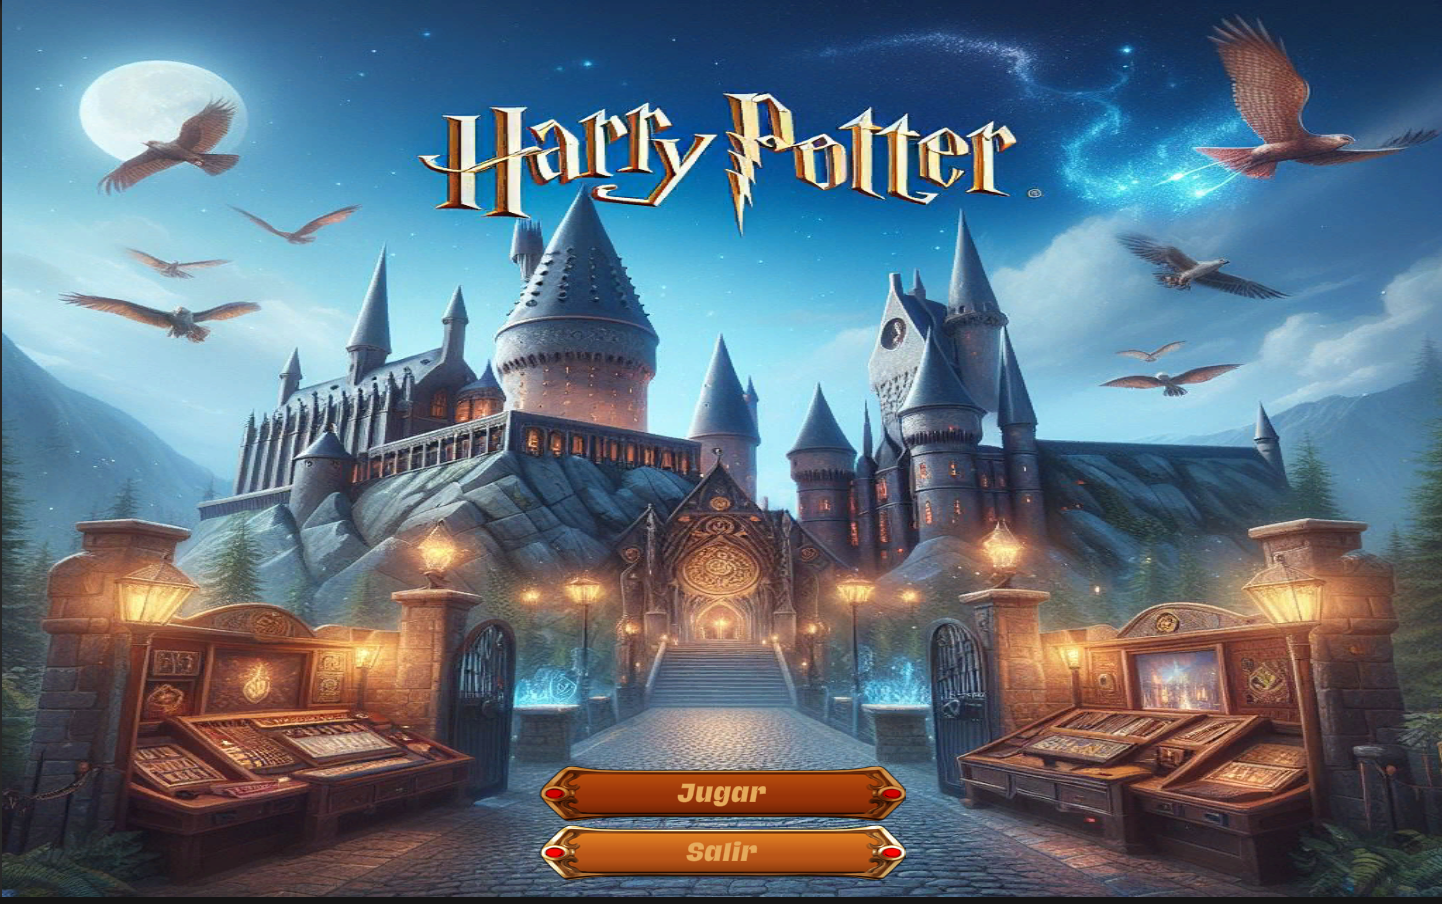
\includegraphics[scale = 0.2]{images/image1.png}
\end{frame}

\begin{frame}{\textcolor{plata}{Escena: Logear}}
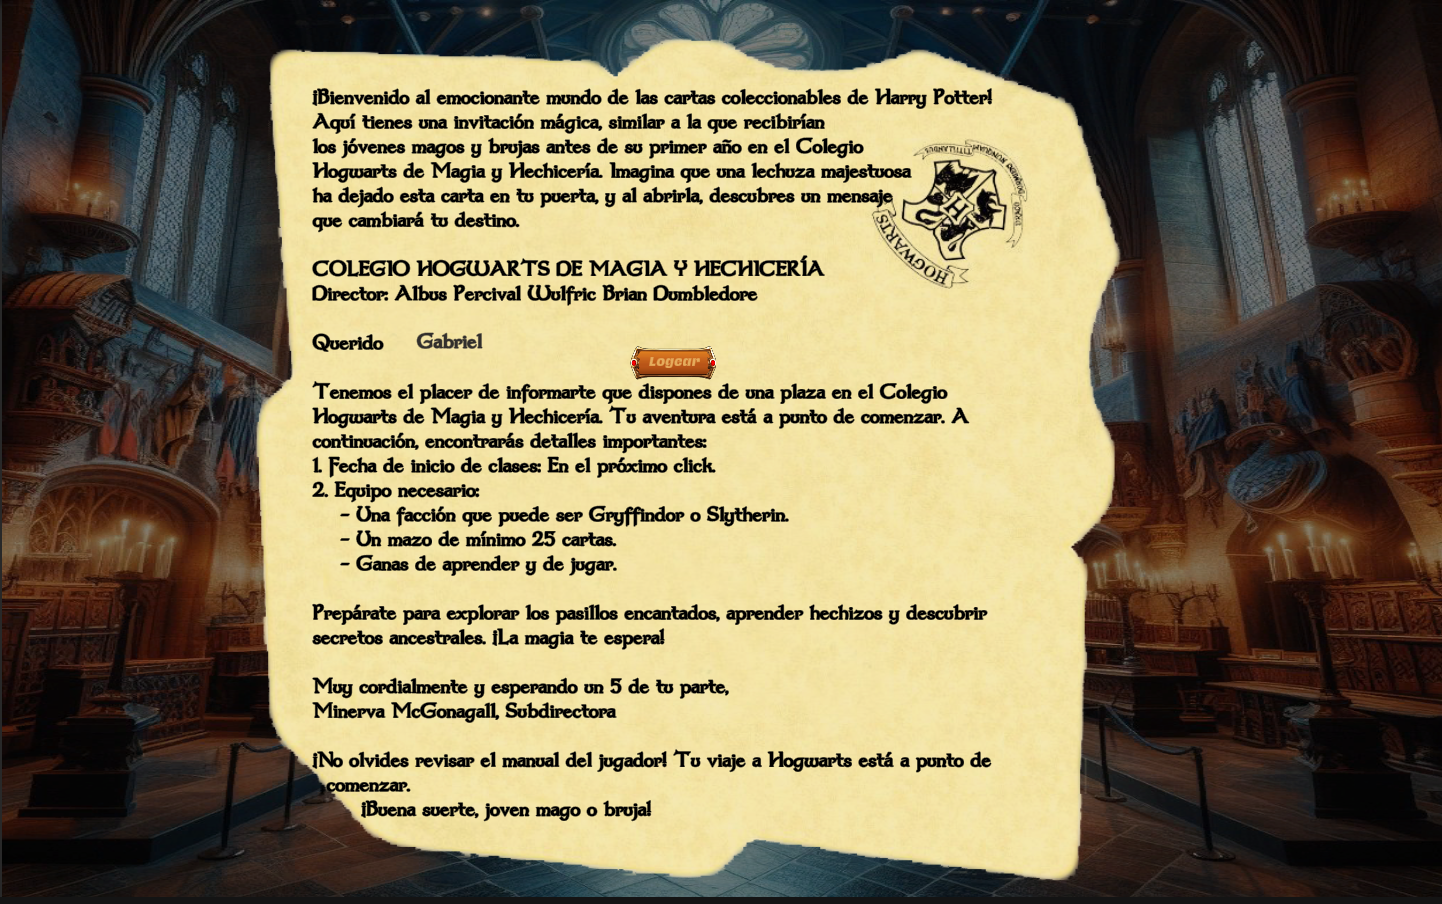
\includegraphics[scale = 0.2]{images/image2.png}
\end{frame}

\begin{frame}{\textcolor{plata}{Escena: Crear Mazo}}
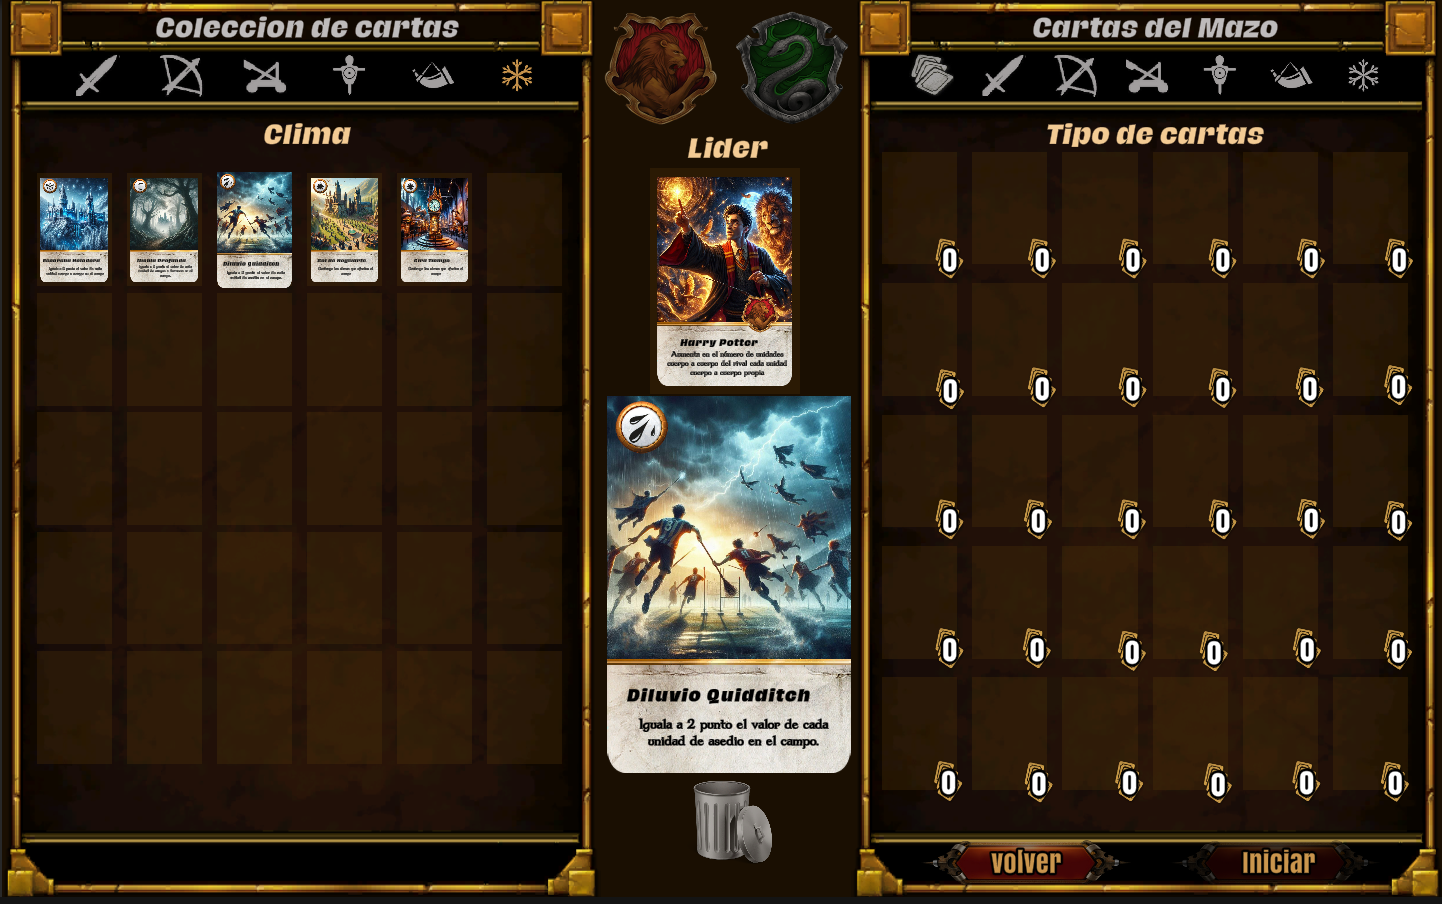
\includegraphics[scale = 0.2]{images/image3.png}
\end{frame}

\begin{frame}{\textcolor{plata}{Escena: Crear Mazo}}
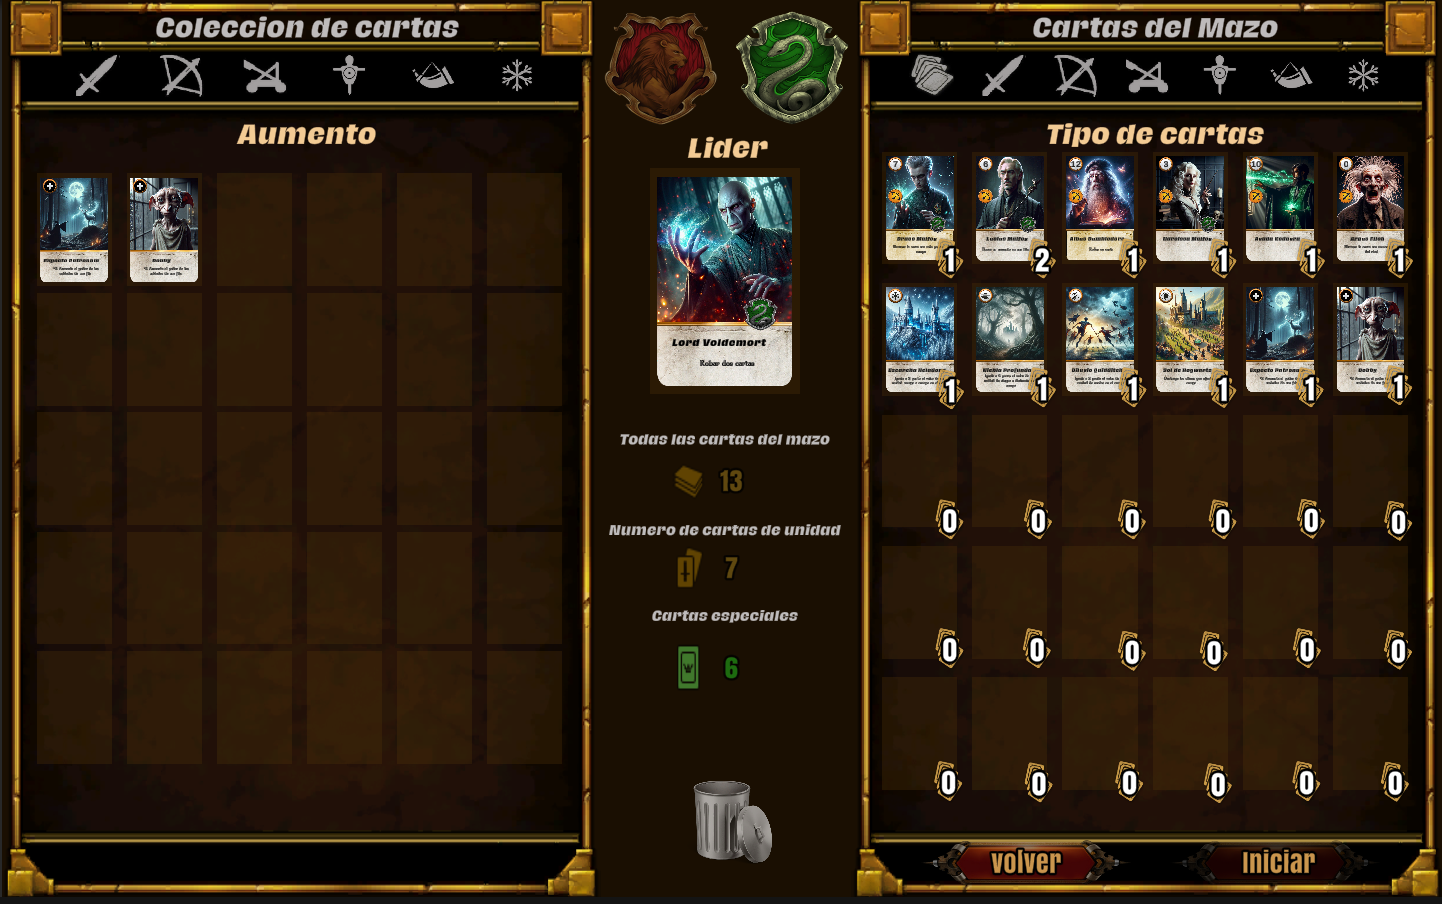
\includegraphics[scale = 0.2]{images/image4.png}
\end{frame}

\begin{frame}{\textcolor{plata}{Escena: Crear Mazo}}
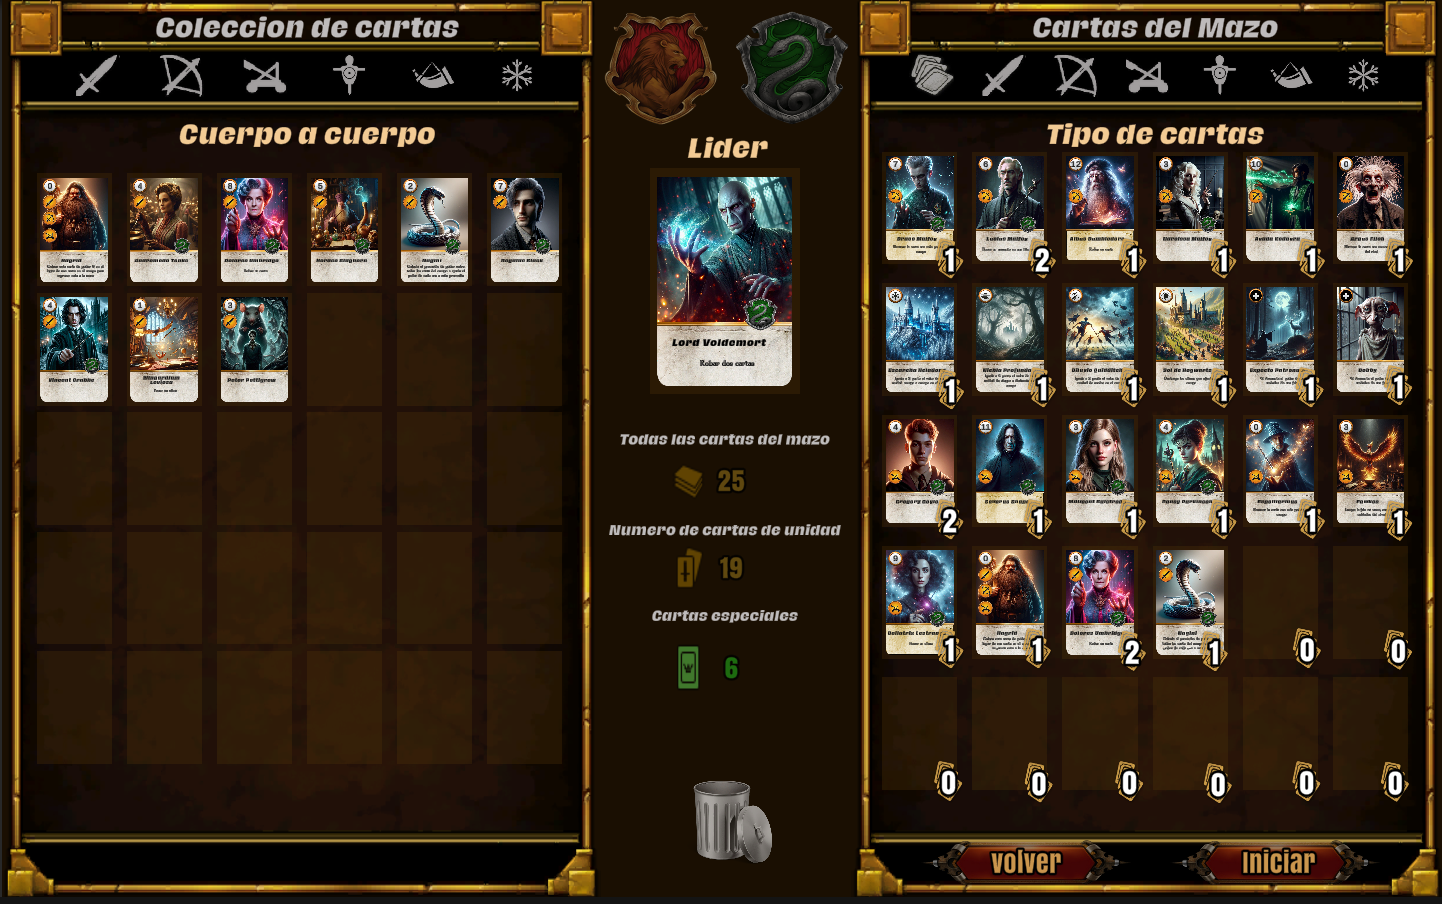
\includegraphics[scale = 0.2]{images/image5.png}
\end{frame}

\begin{frame}{\textcolor{plata}{Escena: Juego}}
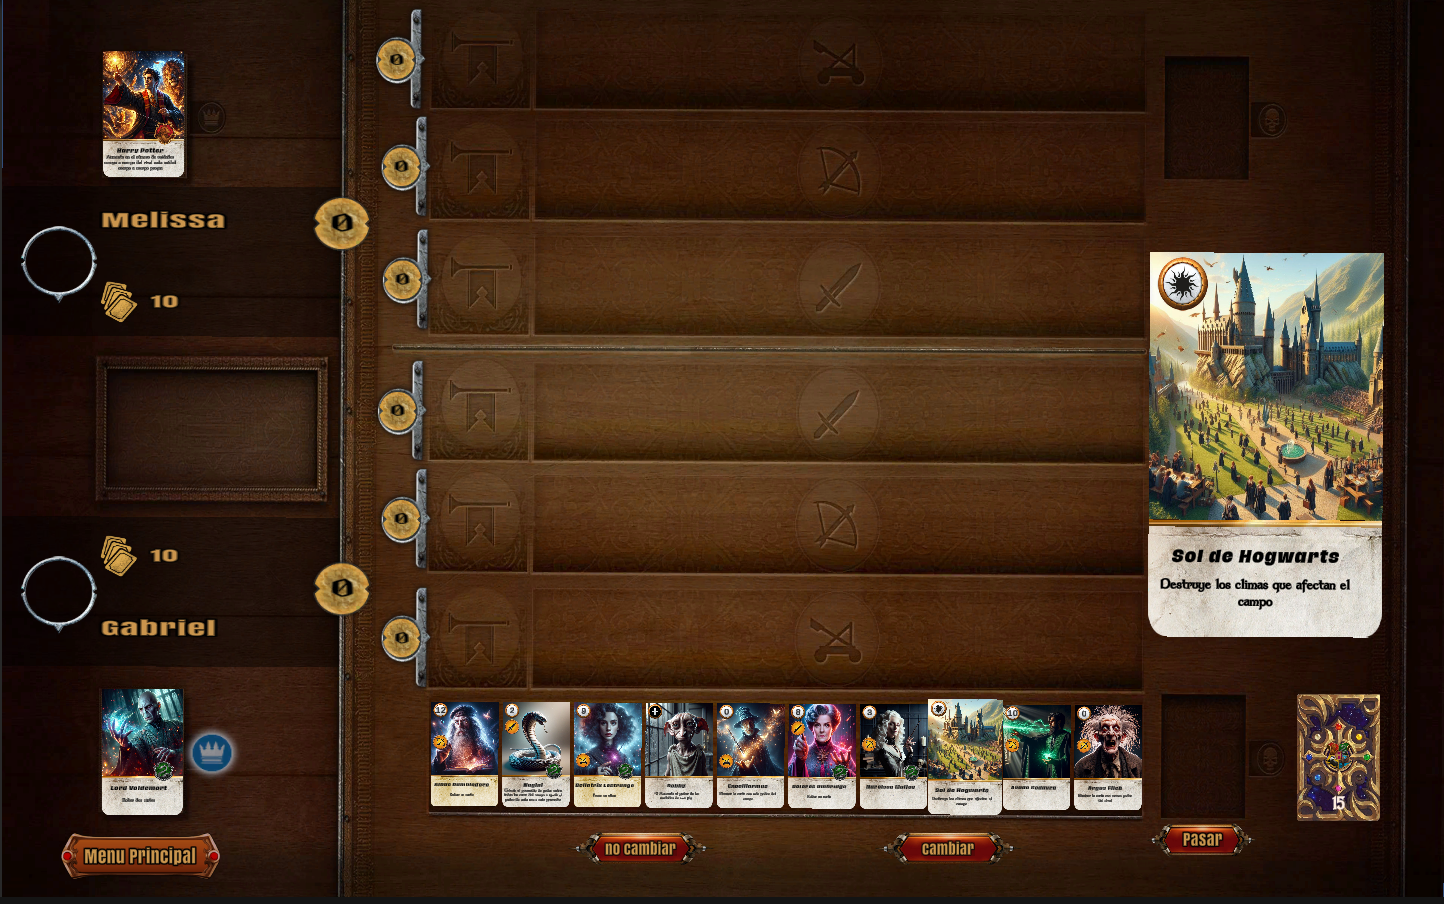
\includegraphics[scale = 0.2]{images/image6.png}
\end{frame}

\begin{frame}{\textcolor{plata}{Escena: Juego}}
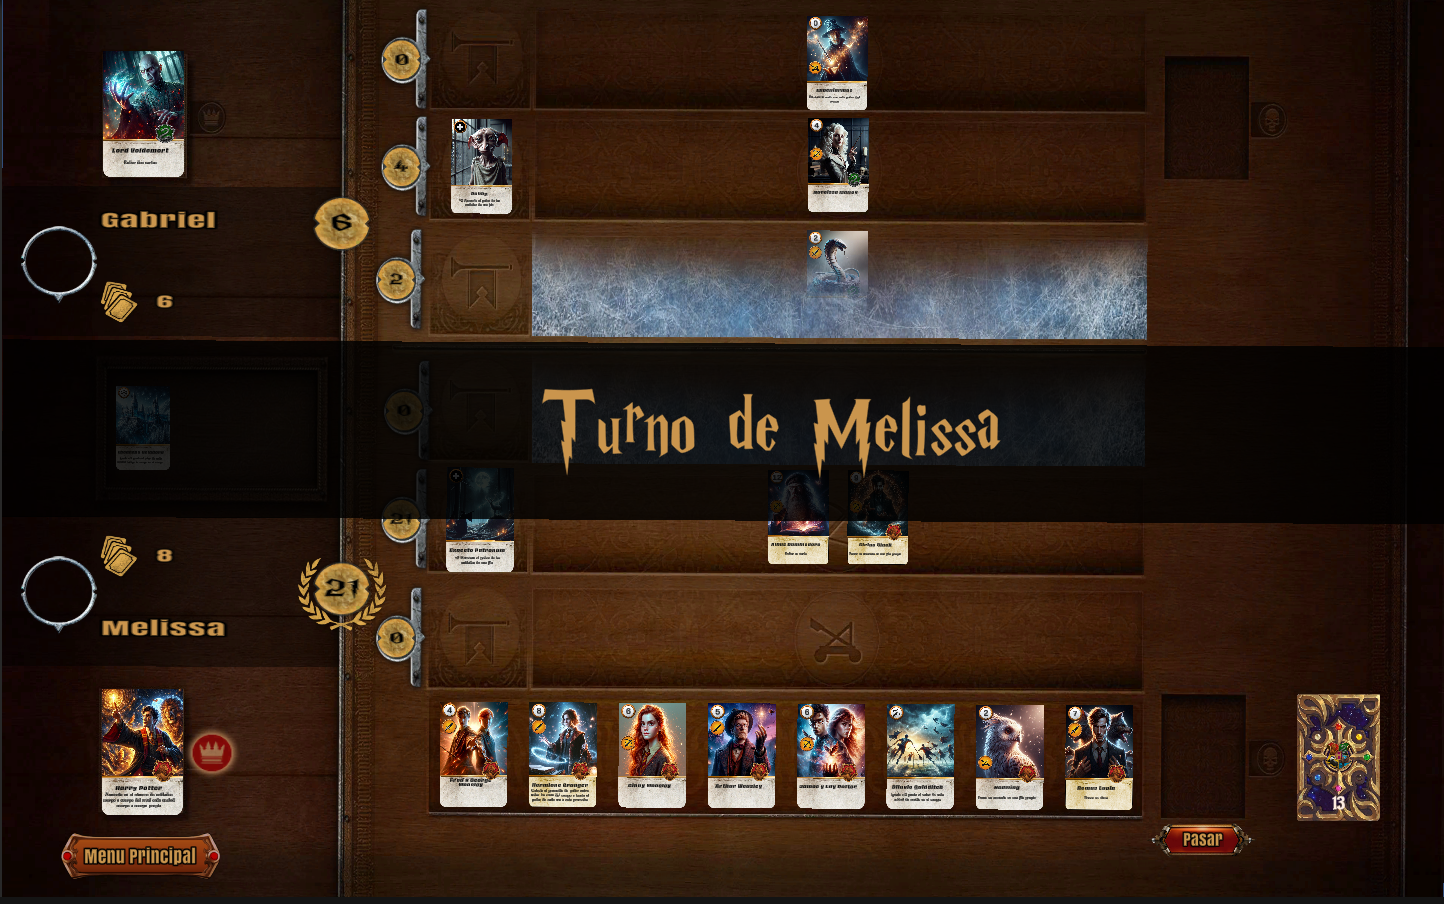
\includegraphics[scale = 0.2]{images/image7.png}
\end{frame}

\begin{frame}{\textcolor{plata}{Escena: Juego}}
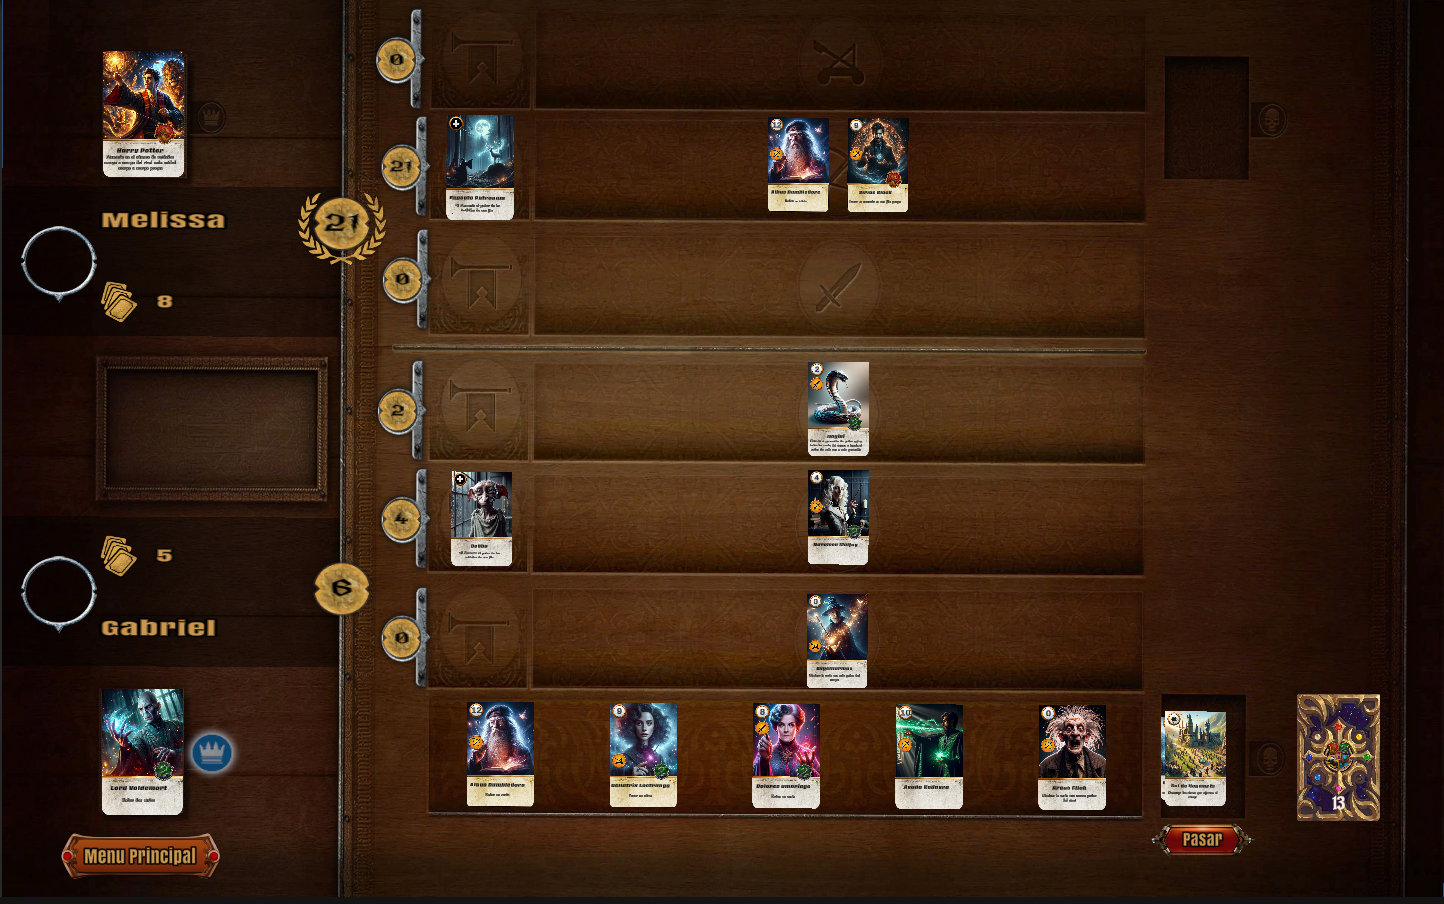
\includegraphics[scale = 0.2]{images/image8.png}
\end{frame}

\begin{frame}{\textcolor{plata}{Escena: Juego}}
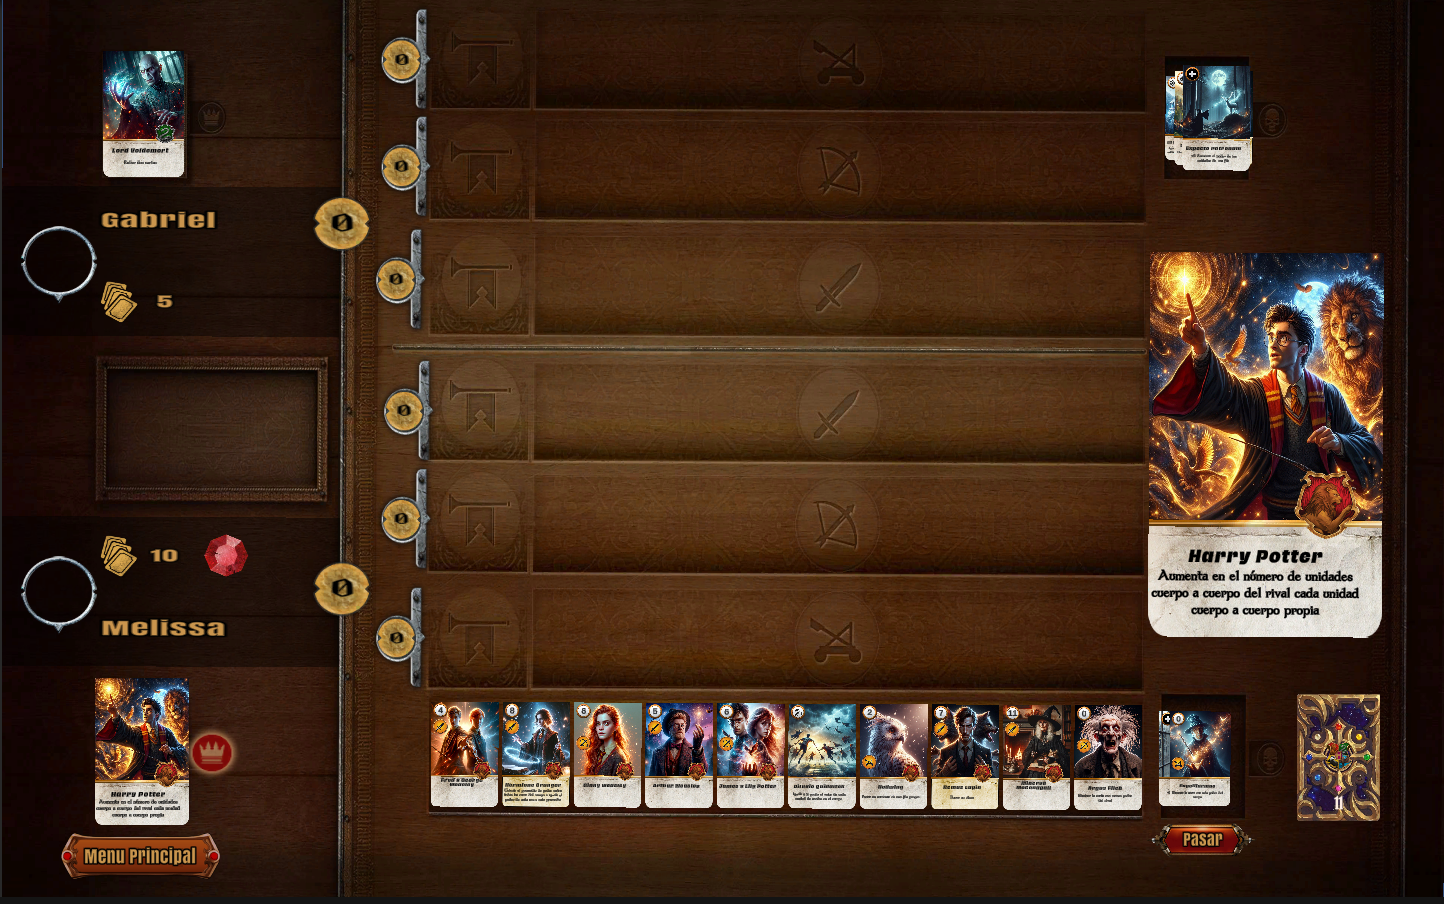
\includegraphics[scale = 0.2]{images/image9.png}
\end{frame}

\end{document}